\section{Electric Fields}
Types of particles
\begin{itemize}
\item proton: charge $+e$
\item electron: charge $-e$
\item $\alpha$-particle: charge $+2e$
\end{itemize}

\begin{defn}{Coulomb’s Law}{}
Electric force between two \underline{point charges} is proportional to the product of the charges and inversely proportional to the square of their separation.
\begin{equation}
\va{F} = k\frac{Qq}{r^2}\hat{\vb{r}}
\end{equation}
where the constant of proportionality is 
\[ k=\frac{1}{4\pi\epsilon_0} \]
where \textbf{permittivity of free space} $\epsilon_0 = 8.85 \times 10^{-12}$ \unit{F.m^{-1}} and can be taken to be equal to that of air unless specified otherwise.
\end{defn}

\begin{remark}
Electric force is repulsive when $Qq>0$ and attractive when $Qq<0$.
\end{remark}

\textbf{Principle of Superposition}: When more than two charges are
present, net force on any one charge is the vector sum of the forces exerted on it by the other charges. For example, if three charges are present, the resultant force experienced by $q_3$ due to $q_1$ and $q_2$ is
\[ \va{F}_3 = \va{F}_{13} + \va{F}_{23} \]
To generalise, for a system of $n$ charges, the net force experienced by the $j$-th particle is
\[ \va{F}_j = \sum_{i=1,i\neq j}^n\va{F}_{ij} \]

\begin{defn}{Electric field}{}
Region of space where a charge experiences an electric force.
\end{defn}

Representation of electric field using \textbf{field lines} (lines of force):
\begin{itemize}
\item An electric field line indicates the direction of the force a positive charge would experience if it is placed at that point in the field (at a normal to surface of charge).
\item The number of field lines per unit cross-sectional area is proportional to the \textbf{electric field strength}.
\item Electric field lines are directed away from positive to negative charges, never intersect each other, and are never created or annihilated in vacuum.
\end{itemize}

\begin{defn}{Electric field strength $\va{E}$}{}
Electric force per unit positive charge on a \emph{small test charge} placed at that point.
\begin{equation} \va{E}=\frac{F}{q}=k\frac{Q}{r^2} \end{equation}
\end{defn}

\begin{remark}
We take charge $q$ to be infinitesimally small so that the field it generates does not disturb that of the ``source charge'', i.e. charge $Q$.
\end{remark}

Comparison between electric field and gravitational field:
\begin{itemize}
\item Qualitative aspect: Gravitational force results from interaction between masses; electric force results from interaction between charges.
\item Quantative aspect: Both fields are inverse square law fields.
\end{itemize}

\begin{defn}{Electric potential $V$}{}
Work done per unit positive charge by an external force in bringing a \emph{small test charge} from infinity to that point.
\begin{equation} V=\frac{W}{q}=k\frac{Q}{r} \end{equation}
where $W$ is the work done on the charge.
\end{defn}

Positive charges move from places of high potential to lower potential, EPE increases.

Negative charges move from places of low potential to higher potential, EPE decreases.

\begin{defn}{Electric potential energy $U$}{}
When two point charges $Q$ and $q$ are at a distance $r$ apart, electric potential energy $U$ of the \emph{system of two charges} is given by 
\begin{equation} U=qV=k\frac{Qq}{r} \end{equation}
\end{defn}

\begin{remark}
EPE can be negative, if one charge is positive and the other is negative.
\end{remark}

\subsection{Parallel plates}
\begin{figure}[H]
    \centering
    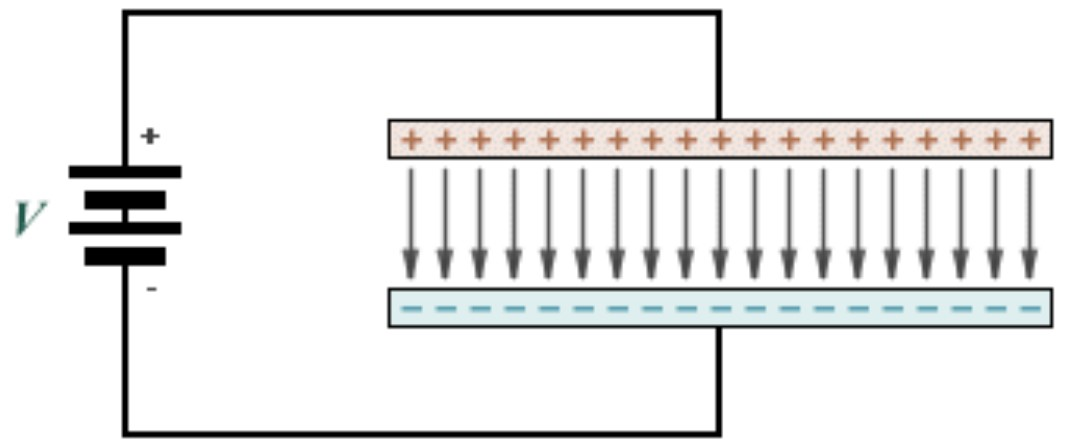
\includegraphics[width=8cm]{images/parallel_plates.jpg}
\end{figure}

Electric field set up is uniform, hence electric field strength $E$ is constant. Thus $F=qE$.

\begin{equation}
E = \frac{|\Delta V|}{d}
\end{equation}
where $|\Delta V|$ is the potential difference across the plates, $d$ is the separation of the plates.

\subsubsection{Charge Moving Perpendicularly to an Electric Field}
\begin{figure}[H]
    \centering
    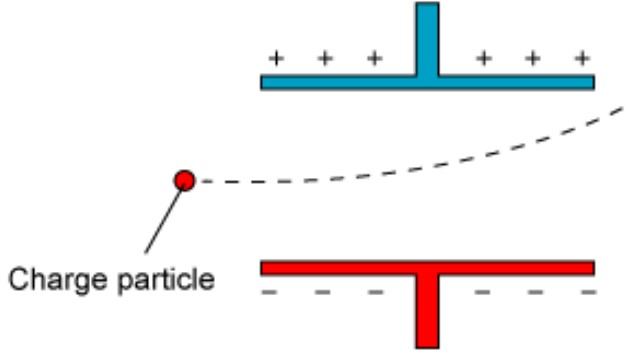
\includegraphics[width=8cm]{images/parallelplates_parabolic.jpg}
\end{figure}

Motion of charged particle in electric field is \textbf{parabolic} in nature.

\begin{proof}
By Newton's 2nd Law, acceleration is given by
\[ a=\frac{F}{m} = \frac{qE}{m} = \frac{q|\Delta V|}{md} \]
which is constant.

Assuming particle is initially at rest, then velocity is given by 
\[ v = u+at = \frac{qE}{m}t \]

When the particle projection is perpendicular to the direction of the electric field, then motion is in the upward direction (along $y$-axis). Thus displacement in $y$-direction is 
\[ y = ut+\frac{1}{2}at^2 = \frac{qE}{2m}t^2 \]

Since $v=xt$, eliminating time dependence gives us 
\[ y = \frac{qE}{2mv^2}x^2 \]
The $y$-$x$ relation is a parabola. Hence the particle follows a parabolic trajectory.
\end{proof}

\subsubsection{Millikan's oil drop}
Physicist Robert Millikan's experiment involves spraying tiny oil droplets into a vertical chamber with two metal plates on either end. The oil droplets became charged. When they entered the chamber, they began to fall under the influence of gravity. He then stopped the free-falling droplets and reversed their direction of motion by applying a voltage across the two metal plates. 

He measured the velocity of a single oil droplet in the electric field to determine the electrical force $F$ acting on it. This allowed him to determine the charge on the oil droplet, since $q=\frac{F}{E}$.

\begin{figure}[H]
    \centering
    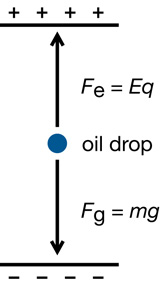
\includegraphics[width=3cm]{images/oil-droplet_free_body_diagram.jpg}
\end{figure}

By measuring the charge of many droplets and comparing them, he reasoned that the smallest difference in charge among all the droplets would be due to the presence of one extra electron. That small difference in charge would then be equal to the charge of a single electron or the elementary charge. He then discovered that the charges of the oil droplets were always integer multiples of $1.60 \times 10^{-19}$ \unit{C}. He reasoned this must be the charge of a single electron, a value that is referred to as the \textbf{elementary unit of charge}.

% https://www.lancaster.ac.uk/media/lancaster-university/content-assets/images/physics/lab-in-a-box/LabInABox_Milikans.pdf
\pagebreak

\subsection*{Problems}
\begin{prbm}
Josiah bought a small engagement ring of mass $m = 1.00 \times 10^{-3}$ \unit{kg}, which he wanted to present to his fianc\'{e}e in a box with a square base of side length $s = 0.100$ \unit{m} and negligible height. On opening the box, he wanted the ring to hover a short distance above its centre. To achieve this, he hid a positive point charge $+q$ under the centre of the box and applied the same positive charge $+q$ to the ring. To constrain the ring to hover directly above the centre of the box, he tied four thin inextensible strings of length $l = 0.120$ \unit{m} to the ring and secured them to the four corners of the box. 

Suppose the ring is small enough to be approximated by a point charge. What is the minimum charge $q$ required to ensure the four strings remain taut while the ring hovers above the box?

\textit{Leave your answer to 3 significant figures in units of $\mu$ \unit{C}.}

\begin{figure}[H]
    \centering
    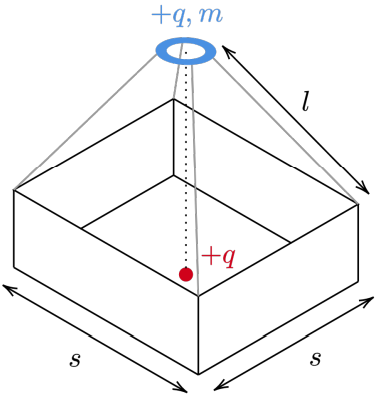
\includegraphics[width=6cm]{images/A_Simple_Proposal.png}
\end{figure}
\end{prbm}

\begin{solution}
Three types of forces act on the hovering ring: the electrostatic repulsion from the hidden point charge, the weight of the ring, and the tension from the strings. These forces must cancel for the ring to hover in place.

Let $h$ be the height above the box at which the ring hovers, and let us define the downwards direction to be positive. As shown in the diagram, the electrostatic repulsion is $-\dfrac{q^2}{4\pi\epsilon_0h^2}$ while the weight from the ring is $+mg$.

Since the net (downwards) force from the tension of the four strings, T, balances the gravitational and electrostatic forces on the ring, we have:
\[ T=\frac{q^2}{4\pi\epsilon_0h^2}-mg \]

\begin{figure}[H]
    \centering
    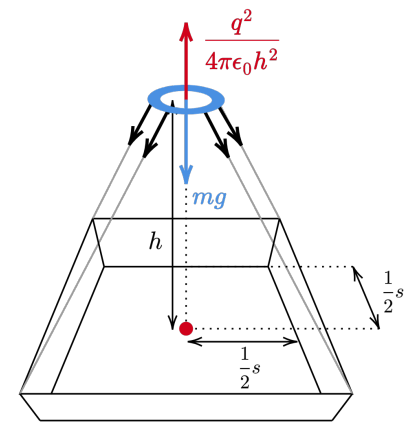
\includegraphics[width=8cm]{images/A_Simple_Proposal1.png}
\end{figure}

For the strings to remain taut, the tensions in the string must be non-negative, which implies that:
\[ T=\frac{q^2}{4\pi\epsilon_0h^2}-mg\ge0 \implies q^2\ge4\pi\epsilon_0mgh^2 \]
From the same diagram above and Pythagoras’s theorem, we can infer that:
\[ l^2=\brac{\frac{s}{2}}^2+\brac{\frac{s}{2}}^2+h^2 \implies h=\sqrt{l^2-\frac{s^2}{2}} \]

Substituting this expression for $h$ into the previous equation and isolating $q$ implies that the charge must be at least:
\begin{align*}
q &\ge \sqrt{4\pi\epsilon_0mg\brac{l^2-\frac{s^2}{2}}} \\
\Aboxed{q &\approx 0.101\:\mu\unit{C}}
\end{align*}
\end{solution}

\pagebreak